\vspace{-0.2cm}
\section{\methodname: Calibrated Q-Learning}
\label{sec:empirical-method}
\vspace{-0.25cm}
Our approach, calibrated Q-learning (\methodname) aims to learn a conservative and calibrated value function initializations from an offline dataset. To this end, \methodname\ builds on CQL from Chapter~\ref{chapter:cql} and then constrains the learned Q-function to produce Q-values larger than the Q-value of a reference policy $\mu$ per Definition~\ref{cond:calibration}. In principle, our approach can utilize many different choices of reference policies, but for developing a practical method, we simply utilize the behavior policy as our reference policy.  

\niparagraph{\textbf{Calibrating CQL.}} We can constrain the learned Q-function $Q^\pi_\theta$ to be larger than $V^\mu$ via a simple change to the CQL training objective from Chapter~\ref{chapter:cql}: masking out the push down of the learned Q-value on out-of-distribution (OOD) actions in CQL if the Q-function is not calibrated, i.e., if $\mathbb{E}_{a \sim \pi}\left[Q^\pi_\theta(\bs, \mathbf{a})\right] \leq V^\mu(\bs)$. \methodname\ modifies the CQL regularizer, $\mathcal{R}(\theta)$ in this manner: 
\begin{align}
\label{eqn:cal_ql_training}
\!\!\!\!\!\!\mathbb{E}_{\bs \sim \mathcal{D}, \mathbf{a} \sim \pi} \brac{{\color[HTML]{B85450}{\max \left( Q_\theta(s,a), V^\mu(s) \right)}} } - \mathbb{E}_{\bs, \mathbf{a} \sim \mathcal{D}}\left[Q_\theta(\bs,\mathbf{a})\right],
\end{align}
where the changes from standard CQL are depicted in {\color[HTML]{B85450} red}. As long as $\alpha$ in CQL is large, for any state-action pair where the learned Q-value is smaller than $Q^\mu$, the Q-function in Equation~\ref{eqn:cal_ql_training} will upper bound $Q^\mu$ in a tabular setting. Of course, as with any practical RL method, with function approximators and gradient-based optimizers, we cannot guarantee that we can enforce this condition for every state-action pair, but in our experiments, we find that Equation~\ref{eqn:cal_ql_training} is sufficient to enforce the calibration in expectation over the states in the dataset.         

\begin{wrapfigure}{r}{0.65\linewidth}
\centering
\vspace{-0.2cm}
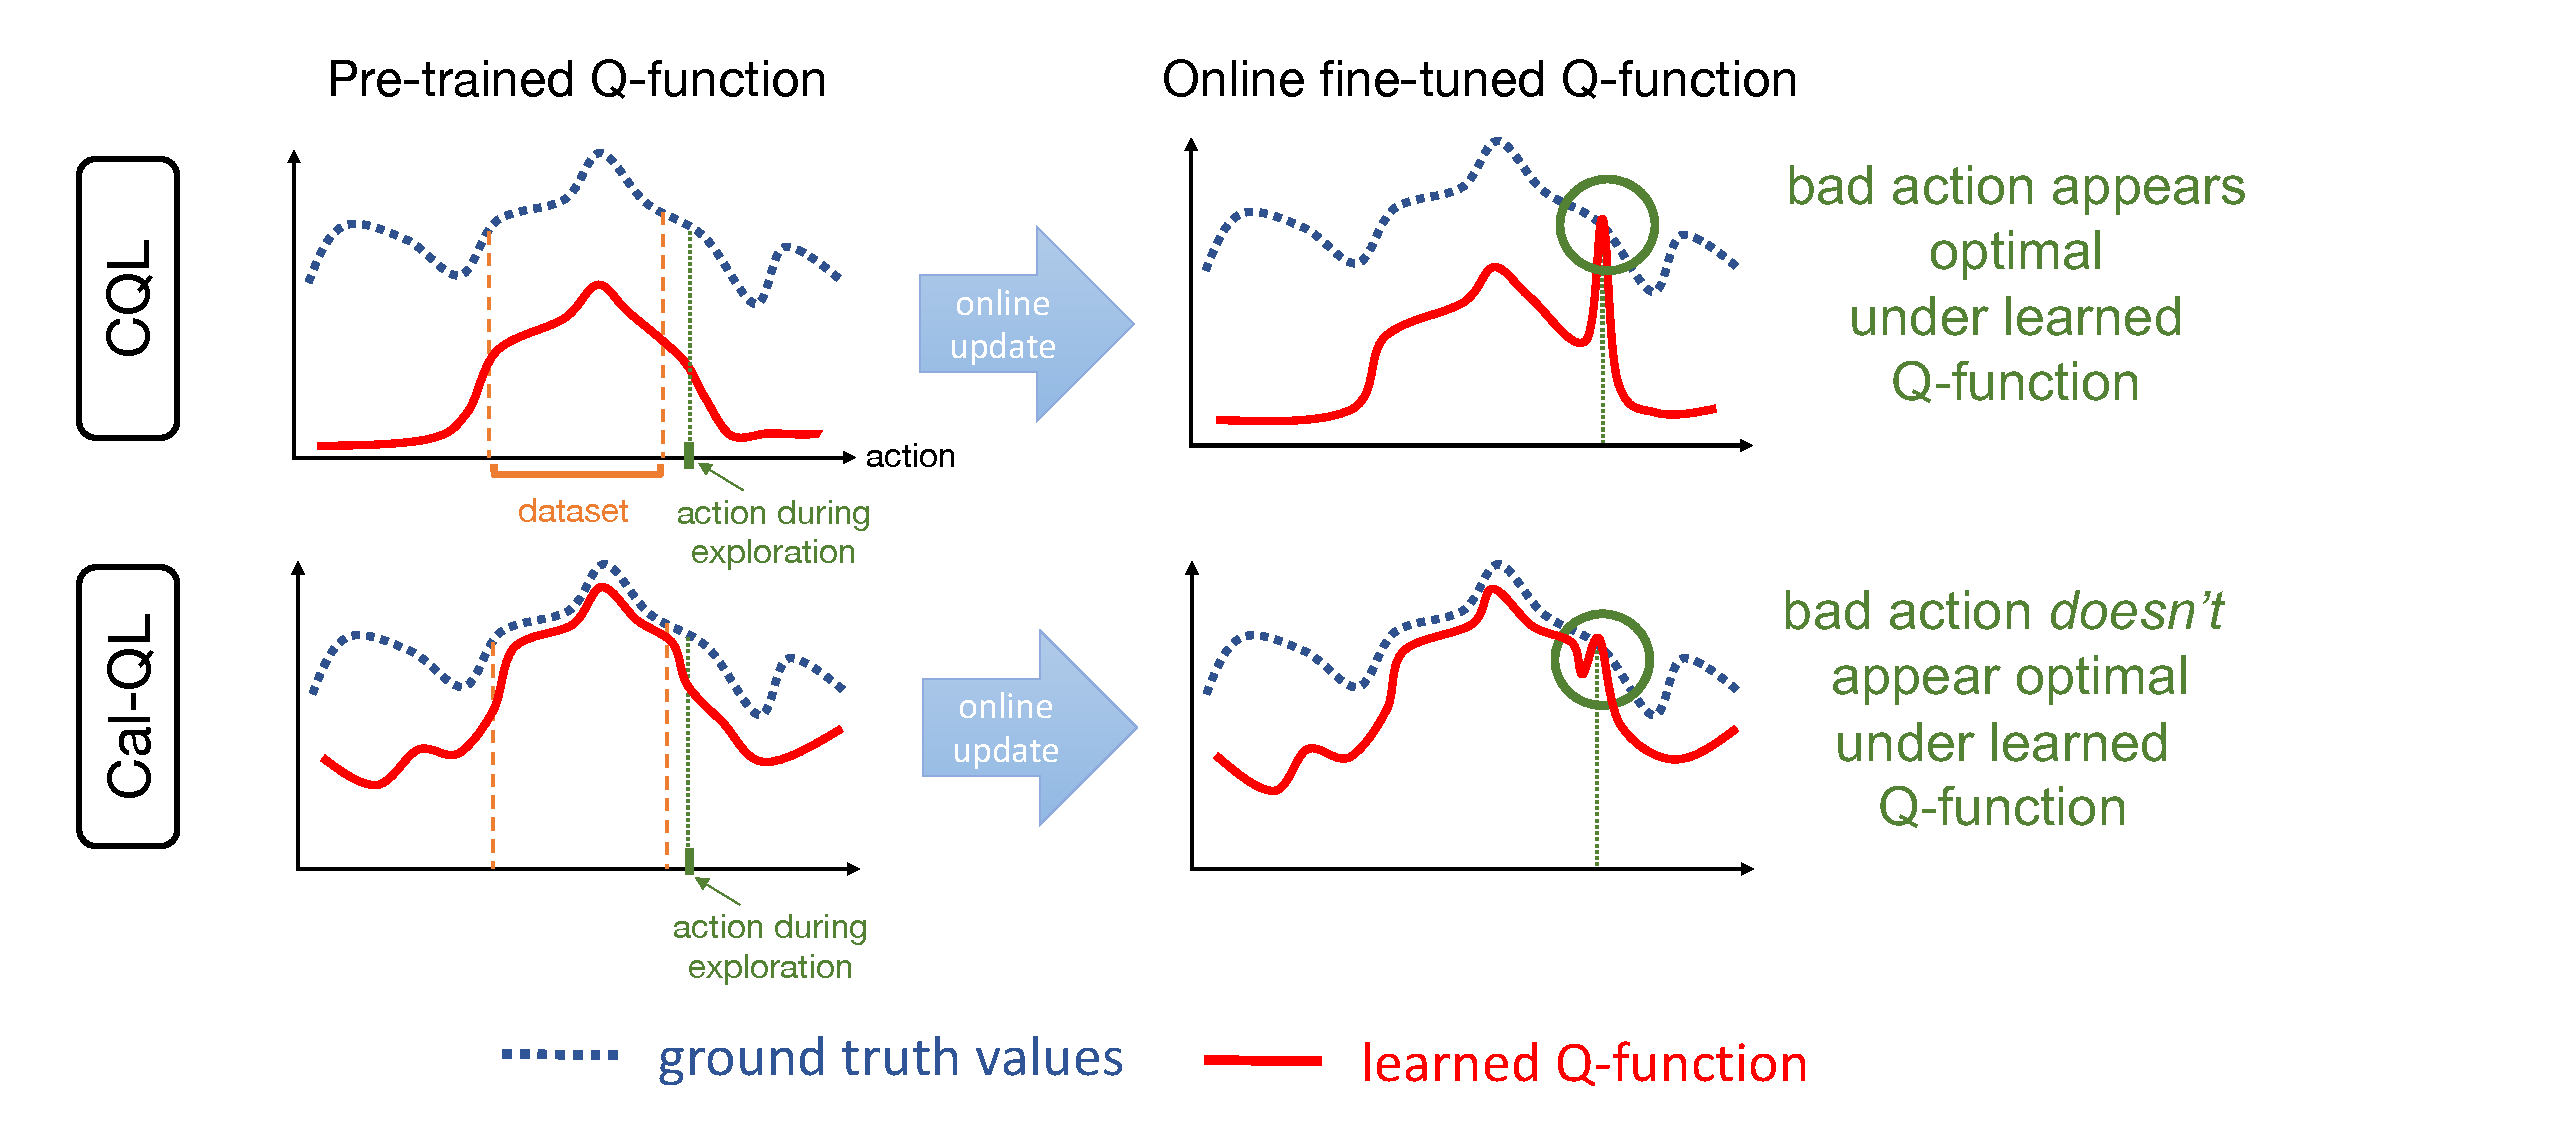
\includegraphics[trim={0 0 2.7cm 0},clip,width=0.98\linewidth]{chapters/cal_ql/figs-sample/figure_for_calql_final.pdf}
\vspace{-0.2cm}
\caption{
\footnotesize{\textbf{Intuition behind policy unlearning with CQL and the idea behind \methodname.} The plot visualizes a slice of the learned Q-function and the ground-truth values for a given state. Erroneous peaks on suboptimal actions (x-axis) arise when updating CQL Q-functions with online data. This in turn can lead the policy to deviate away from high-reward actions covered by the dataset in favor of erroneous new actions, resulting in deterioration of the pre-trained policy. In contrast, \methodname\ corrects the scale of the learned Q-values by using a reference value function, such that actions with worse Q-values than the reference value function do not erroneously appear optimal in fine-tuning.}}
\label{fig:calql_idea}
\vspace{-0.4cm}
\end{wrapfigure}

\niparagraph{\textbf{Pseudo-code and implementation details.}} Our implementation of \methodname\ directly builds on the implementation of CQL from \citet{geng2022jaxcql}. We present a pseudo-code for \methodname\ in Algorithm~\ref{alg:practical_alg}. Additionally, we list the hyperparameters $\alpha$ for the CQL algorithm and our baselines for each suite of tasks in Appendix \ref{app:calql_hyperparam}. Following the protocol in prior work~\citep{kostrikov2021iql,song2023hybrid}, the practical implementation of \methodname\ trains on a mixture of the offline data and the new online data, weighted in some proportion during fine-tuning. To get $V^\mu(\bs)$, we can fit a function approximator $Q^\mu_\theta$ or $V^\mu_\theta$ to the return-to-go values via regression, but we observed that also simply utilizing the return-to-go estimates for tasks that end in a terminal was sufficient for our use case. We show in  Section~\ref{sec:calql_experiments}, how this simple change to the objective drastically improves over prior fine-tuning results.

\vspace{-0.2cm}